% !TeX spellcheck = it_IT
\newpage
\section{Agenti intelligenti}
L'approccio moderno dell'IA (AIMA) è quello di costruire degli \textbf{agenti intelligenti}. La visione ad agenti offre n quadro di riferimento e una prospettiva più generale. È utile anche perché è \textbf{uniforme}.
\begin{center}
<<<<<<< HEAD
	\includegraphics[scale=0.25]{images/agente.png}
=======
	\includegraphics[scale=0.25]{agente.png}
>>>>>>> bce1ea70f19c32bbad14941d401a08b8dc8915cc
\end{center}
Noi ci concentreremo sul programma che sta al centro dell'agente e che consiste in un ciclo di percezione-azione.
\subsection{Caratteristiche}
Un agente ha alcune caratteristiche:
\begin{itemize}
	\item \textbf{Situati}: ricevono \emph{percezioni} da un ambiente e agiscono mediante \textbf{azioni} (attuatori)
	
\end{itemize}

\subsubsection{Percezioni e azioni}
Le percezioni corrispondono agli \textbf{input} dai sensori. La \textbf{sequenza percettiva} sarà la storia completa delle percezioni.\\
La scelta dell'azione è \emph{funzione} unicamente della sequenza percettiva ed è chiamata \textbf{funzione agente}.\\
Il compito dell'IA è costruire il programma agente.
\begin{center}
<<<<<<< HEAD
	\includegraphics[scale=0.2]{images/architettura_astratta.png}
	\includegraphics[scale=0.2]{images/agente_finanziario.png}
=======
	\includegraphics[scale=0.2]{architettura_astratta.png}
	\includegraphics[scale=0.2]{agente_finanziario.png}
>>>>>>> bce1ea70f19c32bbad14941d401a08b8dc8915cc
\end{center}
%TODO Caption

\subsection{Agente razionale}
\begin{definition}[Agente razionale]
	Un agente razionale interagisce con il suo ambiente in maniera \textbf{efficace} (fa la cosa giusta).
\end{definition}
Si rende quindi necessario un \textbf{criterio di valutazione} oggettivo dell'effetto delle azioni dell'agente. La valutazione della prestazione deve avere le seguenti caratteristiche:
\begin{itemize}
	\item \textbf{Esterna}
	\item 
	\item 
\end{itemize}
\begin{definition}[Agente razionale]
	Per ogni sequenza di percezioni compie l’azione che massimizza il valore atteso della
	misura delle prestazioni, considerando le sue percezioni passate e la sua conoscenza pregressa.
\end{definition}
\begin{observation}
	Si basa sulla razionalità e non sull'onniscenza e onnipotenza: non conosce alla perfezione il futuro ma può apprendere e hai dei limiti nelle sue azioni.
\end{observation}

Raramente tutta la conoscenza sull’ambiente può essere fornita a priori dal programmatore. L’agente razionale deve essere in grado di modificare il proprio comportamento con l’esperienza. Può \textbf{migliorare} esplorando, apprendendo, aumentando l'autonomia per operare in ambienti differenti o mutevoli.

\begin{definition}[Agente autonomo]
	Un agente è autonomo nella misura in cui il suo comportamento dipende dalla sua
	capacità di ottenere esperienza e non dall’aiuto del progettista.
\end{definition}

\subsection{Ambienti}
Definire un problema per un agente significa innanzitutto caratterizzare l'ambiente in cui opera. Viene utilizzata la descrizione \textbf{PEAS}:
\begin{itemize}
	\item \textbf{P}erformance
	\item \textbf{E}nviroment
	\item \textbf{A}ctuators
	\item \textbf{S}ensors
\end{itemize}

\begin{center}
<<<<<<< HEAD
	\includegraphics[scale=0.3]{images/agente_ambiente.png}
=======
	\includegraphics[scale=0.3]{agente_ambiente.png}
>>>>>>> bce1ea70f19c32bbad14941d401a08b8dc8915cc
	%TODO Caption
\end{center}

L'ambiente deve avere le seguenti proprietà:
\begin{itemize}
	\item Osservabilità:
	\begin{itemize}
		\item Se è \textbf{completamente osservabile} l'apparato percettivo è in grado di dare conoscenza completa dell'ambiente o almeno tutto ciò che è necessario per prendere l'azione
		\item Se è \textbf{parzialmente osservabile} sono presenti limiti o inaccuratezze dell'apparato sensoriale
	\end{itemize}
	\item Agente singolo o multi-agente:
	\begin{itemize}
		\item L'ambiente ad agente \textbf{singolo} può anche cambiare per eventi, non
		necessariamente per azioni di agenti
		\item Quello \textbf{multi-agente} può essere \emph{competitivo} (scacchi) o \emph{cooperativo}
	\end{itemize}
	\item Predicibilità:
	\begin{itemize}
		\item \textbf{Deterministico}: quando lo stato successivo è completamente determinato dallo stato corrente e dall’azione (e.g. scacchi)
		\item \textbf{Stocastico}: quando esistono elementi di incertezza con associata probabilità (e.g. guida)
		\item \textbf{Non deterministico}: quando si tiene traccia di più stati possibili risultato dell’azione ma non in base ad una probabilità
	\end{itemize}
	\item Episodico o sequenziale:
	\begin{itemize}
		\item \textbf{Episodico}: quando l’esperienza dell’agente è divisa in episodi atomici
		indipendenti in cui non c'è bisogno di pianificare (e.g. partite diverse)
		\item \textbf{Sequenziale}: quando ogni decisione influenza le successive (e.g. mosse di scacchi)
	\end{itemize}
	\item Statico o dinamico:
	\begin{itemize}
		\item \textbf{Statico}: il mondo non cambia mentre l’agente decide l’azione (e.g cruciverba)
		\item \textbf{Dinamico}: cambia nel tempo, va osservata la contingenza e tardare equivale a non agire (e.g. taxi)
		\item \textbf{Semi-dinamico}: l’ambiente non cambia ma la valutazione dell’agente sì (e.g. scacchi con timer)
	\end{itemize}
	\item Valori come lo stato, il tempo, le percezioni e le azioni possono assumere valori \textbf{discreti} o \textbf{continui}. Il problema è combinatoriale nel discreto o infinito nel continuo.
	\item \textbf{Noto} o \textbf{ignoto}: una distinzione riferita alla conoscenza dell'agente sulle leggi fisiche dell'ambiente (le regole del gioco). È diverso da osservabile.
\end{itemize}

\begin{definition}[Simulatore]
	Un simulatore è uno strumento software che si occupa di:
	\begin{itemize}
		\item Generare stimoli
		\item Raccogliere le azioni in risposta
		\item Aggiornare lo stato
		\item Attivare altri processi che influenzano l'ambiente
		\item Valutare la prestazione degli agenti (media su più istanze)
	\end{itemize}
	Gli esperimenti su classi di ambienti con condizioni variabili sono essenziali per \textbf{generalizzare}.
\end{definition}

\subsection{Programma agente}
L'agente sarà quindi composto da un'architettura e da un programma. Il programma dell'agente implementa la funzione agente $Ag: Percezioni \to Azioni$. 

\begin{lstlisting}
	function Skeleton-Agent (percept) returns action
		static: memory, agent memory of the world
		memory <- UpdateMemory(memory, percept)
		action <- Choose-Best-Action(memory)
		memory <- UpdateMemory(memory, action)
		return action
\end{lstlisting}

\subsubsection{Tabella}
Un agente basato su tabella esegue una scelta come un accesso ad una tabella che associa un'azione ad ogni possibile sequenza di percezioni.\\
Ha una \textbf{dimensione ingestibile}, è difficile da costruire, non è autonomo ed è di difficile aggiornamento (apprendimento complesso).

\subsubsection{Agenti reattivi}
L'agente agisce in base a quello che percepisce senza salvare nulla in memoria.
\begin{center}
<<<<<<< HEAD
	\includegraphics[scale=0.25]{images/agenti_reattivi.png}
=======
	\includegraphics[scale=0.25]{agenti_reattivi.png}
>>>>>>> bce1ea70f19c32bbad14941d401a08b8dc8915cc
\end{center}
\begin{lstlisting}
	function Agente-Reattivo-Semplice (percezione)
		returns azione
		persistent: regole, un insieme di regole
		condizione-azione (if-then)
		stato <- Interpreta-Input(percezione)
		regola <- Regola-Corrispondente(stato, regole)
		azione <- regola.Azione
		return azione
\end{lstlisting}

\subsubsection{Agenti basati su modello}
L'agente ha uno stato che mantiene la storia delle percezioni e influenza il modello del mondo.
\begin{center}
<<<<<<< HEAD
	\includegraphics[scale=0.25]{images/agenti_modello.png}
=======
	\includegraphics[scale=0.25]{agenti_modello.png}
>>>>>>> bce1ea70f19c32bbad14941d401a08b8dc8915cc
\end{center}
\begin{lstlisting}
	function Agente-Basato-su-Modello (percezione)
		returns azione
		persistent: stato, una descrizione dello stato corrente
								modello, conoscenza del mondo
								regole, un insieme di regole condizione-azione
								azione, azione piu recente
		stato <- Aggiorna-Stato(stato, azione, percez., modello)
		regola <- Regola-Corrispondente(stato, regole)
		azione <- regola.Azione
		return azione
\end{lstlisting}

\subsubsection{Agenti con obiettivo}
Fin'ora l'agente aveva un obiettivo predeterminato dal programma. In questo caso invece viene specificato anche il \textbf{goal} che influenza le azioni. Abbiamo quindi più \textbf{flessibilità} ma meno efficienza.
\begin{center}
<<<<<<< HEAD
	\includegraphics[scale=0.25]{images/agenti_obiettivo.png}
=======
	\includegraphics[scale=0.25]{agenti_obiettivo.png}
>>>>>>> bce1ea70f19c32bbad14941d401a08b8dc8915cc
\end{center}

\subsubsection{Agenti con valutazione di utilità}
In questo caso ci sono \textbf{obiettivi alternativi} o più modi per raggiungerlo. L'agente deve quindi decidere verso dove muoversi e si rende necessaria una \textbf{funzione utilità} che associ ad un obiettivo un numero reale. La funzione terrà anche conto della probabilità di successo (\textbf{utilità attesa}).
\begin{center}
<<<<<<< HEAD
	\includegraphics[scale=0.25]{images/agenti_utilita.png}
=======
	\includegraphics[scale=0.25]{agenti_utilita.png}
>>>>>>> bce1ea70f19c32bbad14941d401a08b8dc8915cc
\end{center}

\subsubsection{Agenti che apprendono}
Questo tipo di agente include la capacità di \textbf{apprendimento} che produce cambiamenti al programma e ne migliora le prestazioni, adattando i comportamenti.\\
L'elemento \textbf{esecutivo} è il programma stesso, quello \textbf{critico} osserva e dà feedback ed infine c'è un generatore di problemi per suggerire nuove situazioni da esplorare.
\begin{center}
<<<<<<< HEAD
	\includegraphics[scale=0.25]{images/agenti_apprendono.png}
=======
	\includegraphics[scale=0.25]{agenti_apprendono.png}
>>>>>>> bce1ea70f19c32bbad14941d401a08b8dc8915cc
\end{center}

\subsubsection{Tipi di rappresentazione}
Gli stati e le transizioni possono essere rappresentati in tre modi:
\begin{itemize}
	\item \textbf{Atomica}: solo con gli stati
	\item \textbf{Fattorizzata}: con più variabili e attributi
	\item \textbf{Strutturata}: con l'aggiunta delle relazioni
\end{itemize}
\begin{center}
<<<<<<< HEAD
	\includegraphics[scale=0.35]{images/rappresentazioni.png}
=======
	\includegraphics[scale=0.35]{rappresentazioni.png}
>>>>>>> bce1ea70f19c32bbad14941d401a08b8dc8915cc
\end{center}